\chapter{Results and Discussion}\label{chapter:res}

\section{Mobile performance}\label{res:performance}

\begin{table}[ht]
	\begin{tabularx}{\textwidth}{X|c|cc|cc}
		\hline
		\multirow{2}{*}{\textbf{\thead{Neural Renderer Configuration}}} 
		& \multirow{2}{*}{\textbf{\thead{Input\\ Layout}}} 
		& \multicolumn{2}{c|}{\thead{\textbf{on GPU (ms)}}}
		& \multicolumn{2}{c}{\thead{\textbf{on DSP (ms)}}} \\ 
		\cline{3-6}
		& 
		& \multicolumn{1}{r|}{\thead{application}}
		& \multicolumn{1}{r|}{\thead{DNN\\alone}}
		& \multicolumn{1}{r|}{\thead{application}}
		& \multicolumn{1}{r}{\thead{DNN\\alone}} \\ 
		\hline
		\thead{ResNet18 encoder, 14.3M params}
		& 2-256-256-4 
		& 55-57
		& 49-50
		& 19--21
		& 19--21 \\
		\hline
		\thead{ResNet18 encoder, 14.3M params}
		& 1-256-256-8 
		& 41--43
		& 38--43
		& 16.6 \underline{cap}
		& 3--4 \\
		\hline
		\thead{MobileNetV3 encoder, 6.7M params}
		& 1-256-256-8 
		& 37--38
		& 30--37
		& 16.6 \underline{cap}
		& 3--4 \\
		\hline
		\thead{MobileNetV3 encoder, 6.7M params}
		& 1-512-512-8
		& 115--136
		& 105--130
		& 21--22
		& 13--14 \\
		\hline
		\thead{ResNet18 encoder, 14.5M params}
		& 1-512-512-8
		& 112--136
		& 105--130
		& 21--22
		& 13--14 \\
		\hline
		\thead{MobileNetV2 encoder, 6.6M params}
		& 1-512-512-8
		& 166--181
		& 150--175
		& 19--21
		& 12--13 \\
		\hline
		\thead{EfficientNet-Lite0 encoder, 6.1M params}
		& 1-512-512-16
		& 71--78
		& 65--75
		& 16.6--17
		& 6--7 \\
		\hline
		\thead{ResNet18 encoder, 14.5M params}
		& 1-640-640-16
		& 200--215
		& 190--200
		& 29--31
		& 28--30 \\
		\hline
	\end{tabularx}	
	\centering
	\caption{Neural Renderer's inference performance, reported for different encoder types, memory layout of input data, when executed on either mobile GPU or DSP devices. The input layout is specified by 4 numbers from left to right: number of OpenGL textures where input frame is rasterized, frame height, frame width, effective number of neural channels stored in a single texture. Since OpenGL textures always have 4 channels, the last number bigger than 4 indicates that quantized 8-bit values are packed into a single texture channel to achieve a contiguous memory layout. The performance of "DNN alone" columns is measured by continuously inferring the DNN with constant random input data, thus excluding: mesh inference, rasterization, output rendering in AR, overall mobile interaction. Application performance has software cap of 60 FPS (16.6 ms).}	\label{res:tab:other-solutions}		
\end{table} 

\section{Quantitative analysis}\label{res:metrics}
\section{Qualitative analysis}\label{res:quality}

\begin{figure}[h!]
	\fboxrule=1pt
	\centering
	\begin{subfigure}[b]{0.495\textwidth}
		\centering
		\cfbox{gray}{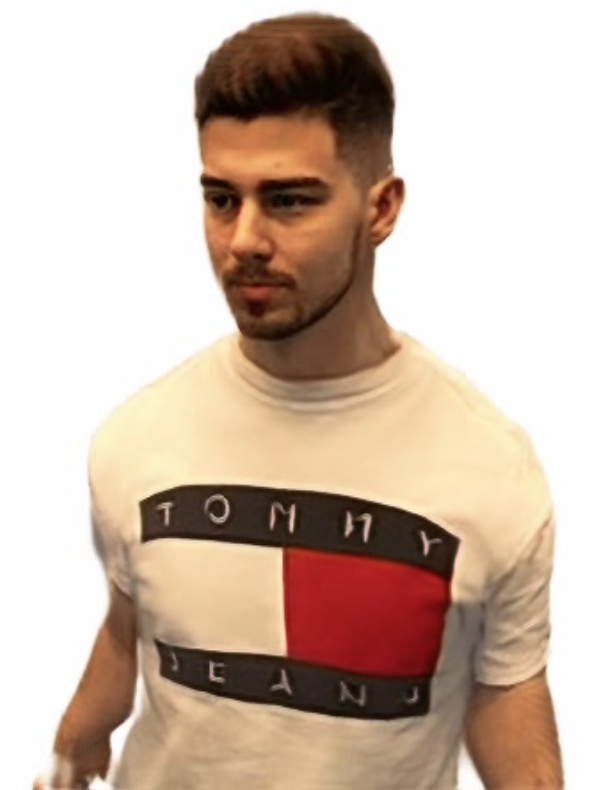
\includegraphics[height=10cm]{\imgfp/example_1}}
		\caption{BNs collect statistics on FB frames}
		\label{res:fig:example}
	\end{subfigure}
	\begin{subfigure}[b]{0.495\textwidth}
		\centering
		\cfbox{gray}{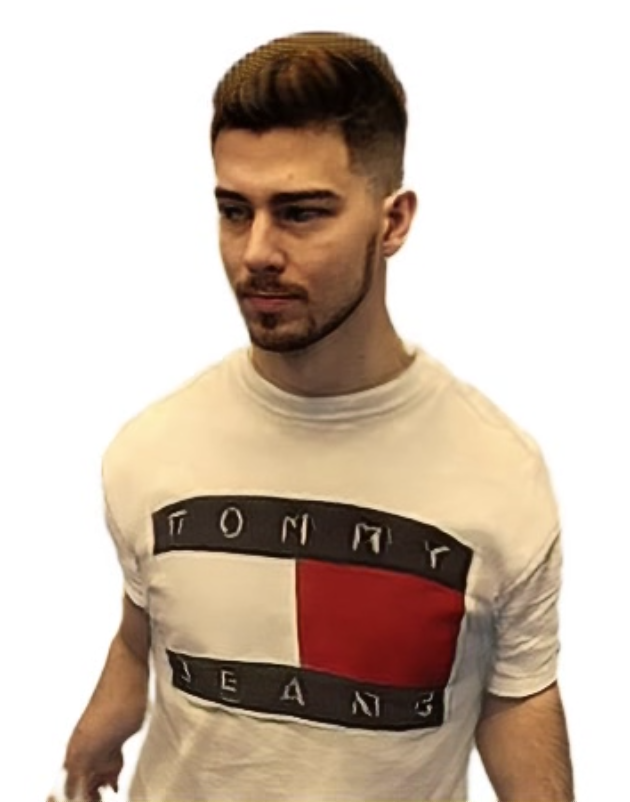
\includegraphics[height=10cm]{\imgfp/example_2}}
		\caption{BNs collect statistics on zoomed frames}
		\label{res:fig:example}
	\end{subfigure}
%	\centering
%	\subcaptionbox{3a\label{fig3:a}}{\includegraphics[width=1.6in]{example-image-c}}\hspace{1em}%
%	\subcaptionbox{3b\label{fig3:b}}{\includegraphics[width=1.6in]{example-image-c}}
	\caption{Example}
	\label{res:fig:example}
\end{figure}

\section{Future work}\label{res:future}

The baseline model \cite{dnn:stylepeople21} is still state-of-the-art in its particular task -- rendering of a full-body avatar using information from a few monocular uncalibrated images, or a video sequence. However, as the original authors point out, it is an optimization-based approach that takes about half a day to converge, and may be impractical in a scenario where users can scan themselves and after a short time be able to use their avatars. The training time can be improved by doing further research on meta-learning, where both architecture and its initialization are sought, so that fine-tuning of it would converge to acceptable results after a very short optimization. On the other hand, a completely new algorithmic feed-forward solution could be proposed, so that a single inference would yield all the necessary data to generate realistic avatars.

Regarding this thesis project, the neural renderer's inference performance could be further improved. For example, we could employ already described approaches of knowledge distillation or neural architecture search, to find an architecture with fewer parameters, but similar visual quality. However, such research efforts are known to be notoriously big, in terms of experimentation and amount of computations. On the other hand, purely algorithmic tricks could be used. The approach of pipelining \cite{mobile:pipelining20} could be used, to split the network into independent stages, with the idea that as soon as a stage finishes computation on the given data, it could pass the data to the next stage, and at the same time accept new input for processing. In the context of the mobile execution, some parts can be executed on different computing units (GPU, DSP) and exchange the data using the shared memory. As was shown in the Section \ref{res:performance}, in the current implementation of the mobile inference there is some idleness of DSP between frames, caused by latency of rasterizing each new frame and sending it to the DNN. More efficient organization of calculations could be researched to minimize this idleness, potentially gaining about 10-15\% of performance. For example, CPU multithreading could be better utilized in the future, or batch inference of the DNN on mobile to improve throughput of data through the computing units.

Improving the quality of synthesized images is also a big field for research. Making small training procedure adjustments as was described in this thesis proved to be ineffective to solve all the current issues with overfitting and randomness. Thus, research on other architectures is yet again more preferable. This also requires to decide on generalization ability of the rendering architecture. On one hand, sticking to one-DNN-one-avatar approach, allows to obtain the full realism for the particular person. A lot of attention is brought to NeRF \cite{dnn:nerf20, dnn:phorhum22} based methods, from which very realistic images can be sampled from many novel views. On the other hand, it would be beneficial if a single DNN could be used to render many avatars, distinguishing them by neural textures. Thus we could place multiple different avatars in a single frame of AR, and generate images of all of them at once. 

Such scenario anticipates the dawn of true telepresence communication, given that mobile devices are already capable of doing real-time DNN inference. However, this would also require to overlook the cropping approach that was used in this thesis to get higher and stable visual quality. Imagine if we were to render two avatars separated by a considerable distance. By using a bounding box that includes both of them to do frustum cropping, both avatars will be quite small in the frame, once again bringing up the necessity for the DNN to be stable on far-views (as in Figure \ref{fig:far_screen_crop}) One way to extend cropping to a multi-avatar scenario, is to use the fact that in OpenGL we can rasterize to a part of an image. Thus, we could compute bounding boxes for each avatar separately, then to distribute the input frame between avatars rasterizations, proportional to used image area in AR (See Figure \ref{fig:multiavatar}). An additional advantage is that we don't need to worry about avatars overlapping, because they will be rasterized one by one, without affecting each other. The time of rasterizing $N$ avatars is still extremely smaller than a DNN inference time. The proportion of areas on the input frame can also be dynamically adjusted to yield better images for nearby avatars, and decreasing quality of far-away ones.

Lastly, the issue of stability in rendering unseen body parts has to be tackled. In this thesis we used a handcrafted solution to replace the corresponding texture parts with content that was seen by the neural renderer. However, we believe, that a more general algorithmic approach could be used, e.g. by inpainting the neural texture with logical content, or by feeding the renderer during training with images that show the missed body parts, even though the training sequence doesn't contain them. These could be images of other people, augmented to match the hair or clothes colors. Or these could be synthesized from some other model that saw these body parts.
%\begin{enumerate}
%	\item To use shared memory between GPU and DSP, to eliminate sending of OpenGL rasterized images between GPU and DSP
%	\item To use bufferization of data to infer DNN in batches (possibly better DSP usage ratio)
%	\item To research on training a single renderer for multiple people, and adjusting mobile inference to fit multiple people simultaneously. We can render multiple avatars in different corners of an input rasterization, regardless of distance in camera space. Then after getting an output image, we can tear apart this image and place corresponding avatars in different places of the AR space.
%	\item To research on completely different neural rendering architectures, since the small adjustments of the current baseline yield little to no benefit
%	\item To find an algorithmic way of solving the issue of unseen body parts during training
%	\item To research on other regularizing techniques to prevent overfitting, without harming high-frequency details learning 
%\end{enumerate}